\documentclass{article} % For LaTeX2e
\usepackage{nips13submit_e,times}
\usepackage{hyperref}
\usepackage{url}
\usepackage{graphicx}
\graphicspath{ {images/} }
%\documentstyle[nips13submit_09,times,art10]{article} % For LaTeX 2.09


\title{Clustering Wikipedia Articles}


\author{
Lane Aasen\\
Department of Computer Science\\
University of Washington\\
Seattle, WA 98105\\
\texttt{aaasen@cs.washington.edu}\\
}

% The \author macro works with any number of authors. There are two commands
% used to separate the names and addresses of multiple authors: \And and \AND.
%
% Using \And between authors leaves it to \LaTeX{} to determine where to break
% the lines. Using \AND forces a linebreak at that point. So, if \LaTeX{}
% puts 3 of 4 authors names on the first line, and the last on the second
% line, try using \AND instead of \And before the third author name.

\newcommand{\fix}{\marginpar{FIX}}
\newcommand{\new}{\marginpar{NEW}}

\nipsfinalcopy % Uncomment for camera-ready version

\begin{document}


\maketitle

\begin{abstract}
Clustering Wikipedia articles using unsupervised learning techniques including K-Means and Latent Dirichlet Allocation (LDA).
\end{abstract}


\section{Dataset}

The provided dataset contains 15,903 Wikipedia articles in tf-idf format. There are 10,574 unique words in this dataset. Each document is represented as a sparse vector with one dimension for each word.

\section{K-Means Clustering}

For the project milestone, I have implemented K-Means clustering on the provided subset of Wikipedia articles.

\subsection{Choosing K}

\subsubsection{Minimizing Distortion}

Given $K$ clusters $C_{1},C_{2},...,C_{K}$ where each cluster is a set of document vectors and $\mu_{i}$ is the centroid of $C_{i}$, the total distortion is defined as follows:

$$\sum_{i=1}^{K}\sum_{d \in C_{i}} ||d - \mu_{i}||^{2}$$

To minimize the distortion, we could set $K$ equal to the number of documents, but then the clusters would be meaningless. We want to choose a $K$ with low distortion that also results in interpretable clusters. Figure 1 shows a plot of $K$ versus total distortion. When $1 \leq K \leq 16$, adding additional clusters has a large impact on the distortion, but once $K > 16$, adding additional clusters has little impact on the distortion. From this alone, it makes sense to set $K=16$ since it provides a good balance of distortion and interpretability.

\clearpage

\begin{figure}[h]
\begin{center}
\framebox{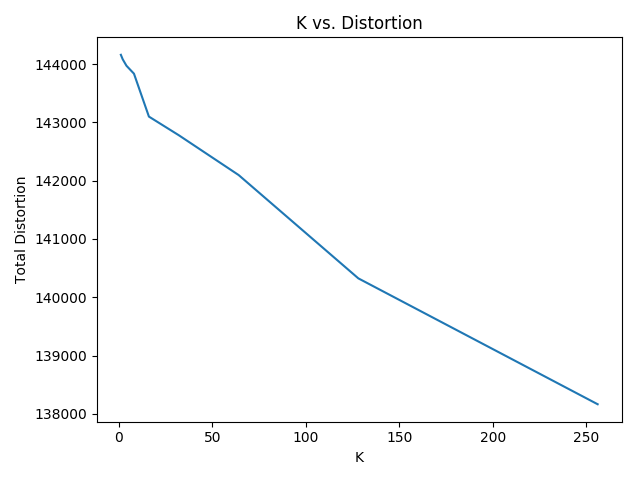
\includegraphics[scale=0.4]{k_vs_distortion}}
\end{center}
\caption{$K$ versus total distortion for $K \in \{1,2,4,...,256\}$}
\end{figure}

\subsection{K and Cluster Size}

As $K$ increases, the clusters become more sparse. Once $K=256$, over half of the clusters have only one document, and are essentially useless. When $K=16$, the median cluster size is 8.5, and the cluster sizes are as follows:

$$[10061, 3013, 1128, 909, 707, 30, 23, 13, 4, 4, 3, 2, 2, 2, 1, 1]$$

Over half of the clusters are very small, and one of the clusters is too large to be interpretable. This indicates that the data has significant outliers and may lack a structure conducive to clustering.

\begin{figure}[h]
\begin{center}
\framebox{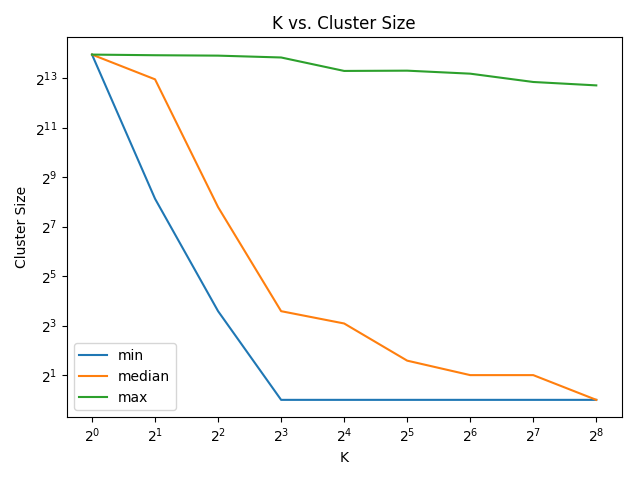
\includegraphics[scale=0.4]{k_vs_cluster_size}}
\end{center}
\caption{$K$ versus minimum, median, and maximum cluster size for $K \in \{1,2,4,...,256\}$ with a $log_{2}$ scale on both axes.}
\end{figure}

\subsection{Exploring Clusters}

Table 1 shows the clusters with at least 10 documents for K-Means clustering with $K=16$. The words in each cluster are the dimensions of the centroid with the largest magnitude. The documents shown are those that are closest to the centroid of the cluster.

Overall, the generated clusters make sense, but there are some points of confusion:

\begin{itemize}
\item The words that make up cluster 0 have little relation to each other. This cluster contains the majority of the documents.
\item Cluster 1 contains churches as well as colleges.
\item Cluster 3 contains documents related to TV shows and sports because both contain the word "season."
\end{itemize}

\subsection{K-Means++}

K-Means++ is a method for selecting initial cluster centers for K-Means. In the normal version of K-Means, initial cluster centroids are selected by sampling random documents from the dataset. This can produce suboptimal clusters, increase time to convergence, and increase variability in clustering performance. K-Means solves this by selecting initial centroids one at a time to minimize distortion.

I implemented K-Means++ and expected it to increase clustering performance considerably. However, I found that it actually had a slightly negative impact on distortion and noticeably increased cluster sparsity. 

\begin{figure}[h]
\begin{center}
\framebox{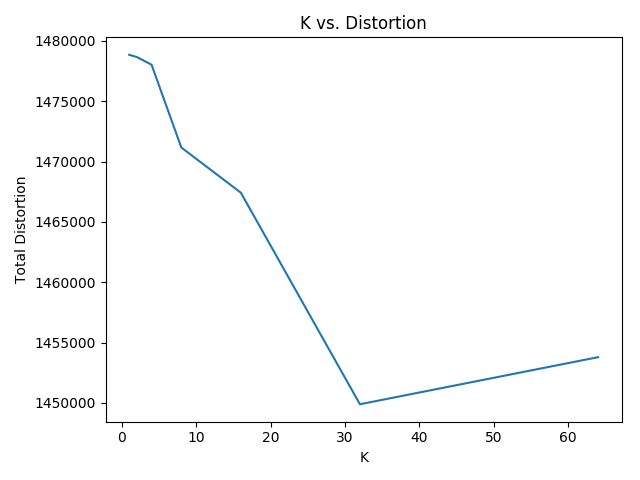
\includegraphics[scale=0.4]{k_vs_distortion_++}}
\end{center}
\caption{$K$ versus total distortion for $K \in \{1,2,4,...,64\}$ using K-Means++.}
\end{figure}


\begin{figure}[h]
\begin{center}
\framebox{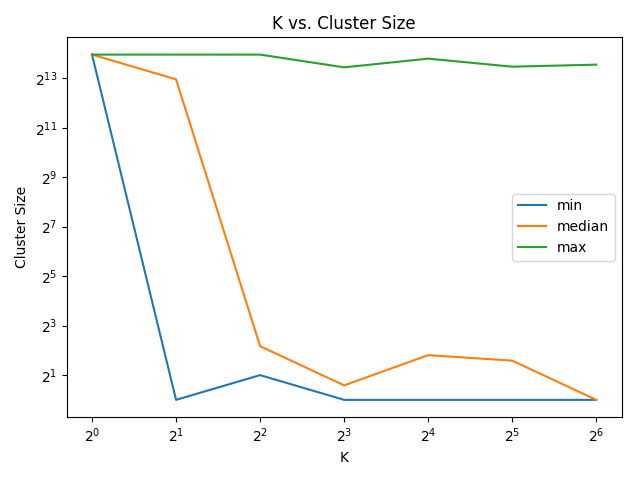
\includegraphics[scale=0.4]{k_vs_cluster_size_++}}
\end{center}
\caption{$K$ versus minimum, median, and maximum cluster size for $K \in \{1,2,4,...,64\}$ with a $log_{2}$ scale on both axes. Using K-Means++.}
\end{figure}

\subsection{Fighting Cluster Sparsity}

After implementing K-Means++ with no success, it became apparent that there was a problem with the underlying data, and not with the clustering algorithm. 

I began to investigate the provided dataset, which was in tf-idf format with no documentation. I found that stop words had been removed from the dataset, but rare words had been left in. Half of the words in the dictionary were used in 16 or fewer datasets (less than 0.1\%). This was the obvious cause of cluster sparsity in the dataset. 

\begin{table}[t]
\caption{10 least common words with the number and percentage of documents that they appear in.}
\label{least-common-words-table}
\begin{center}
    \begin{tabular}{ | c | c | c |}
    \hline
    \textbf{Word} & \textbf{Documents} & \textbf{Percentage of Documents} \\ \hline

frazioni & 0 & 0.0\% \\ \hline 
threeletter & 1 & 0.0062881\% \\ \hline 
budjovice & 1 & 0.0062881\% \\ \hline 
gmina & 1 & 0.0062881\% \\ \hline 
ortsgemeinden & 1 & 0.0062881\% \\ \hline 
headwater & 2 & 0.012576\% \\ \hline 
baronetage & 3 & 0.018864\% \\ \hline 
breaststroke & 3 & 0.018864\% \\ \hline 
voronezh & 3 & 0.018864\% \\ \hline 
rosettes & 3 & 0.018864\% \\ \hline 

\end{tabular}
\end{center}
\end{table}

\begin{table}[t]
\caption{10 most common words with the number and percentage of documents that they appear in.}
\label{most-common-words-table}
\begin{center}
    \begin{tabular}{ | c | c | c |}
    \hline
    \textbf{Word} & \textbf{Documents} & \textbf{Percentage of Documents} \\ \hline

well & 4009 & 25.209\% \\ \hline 
second & 3538 & 22.247\% \\ \hline 
high & 2836 & 17.833\% \\ \hline 
family & 2579 & 16.217\% \\ \hline 
group & 2412 & 15.167\% \\ \hline 
north & 2364 & 14.865\% \\ \hline 
major & 2298 & 14.45\% \\ \hline 
large & 2227 & 14.004\% \\ \hline 
general & 2187 & 13.752\% \\ \hline 
long & 2164 & 13.607\% \\ \hline 

\end{tabular}
\end{center}
\end{table}

\subsection{Effect of Seed on Distortion}

After observing some variability in my plots of K vs Distortion, I decided to investigate the effect of random seeds on distortion.

I found that the choice of seed can have a large impact on cluster quality and distortion. Because of this, it is very important to run K-Means with at least a few different seeds and select the best one. I opted to not do this in the above experiments because it would have been too computationally expensive, but I will try many different seeds when generating the final clusters.

\begin{figure}[h]
\begin{center}
\framebox{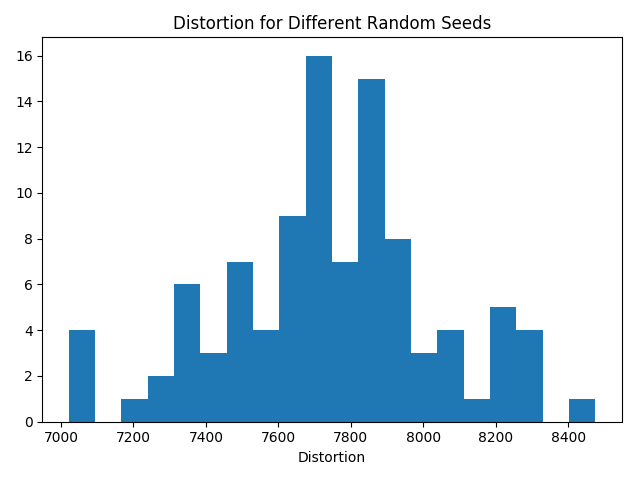
\includegraphics[scale=0.4]{different_init}}
\end{center}
\caption{Distortion using K-Means++ on 100 training documents with different random seeds.}
\end{figure}


\begin{figure}[h]
\begin{center}
\framebox{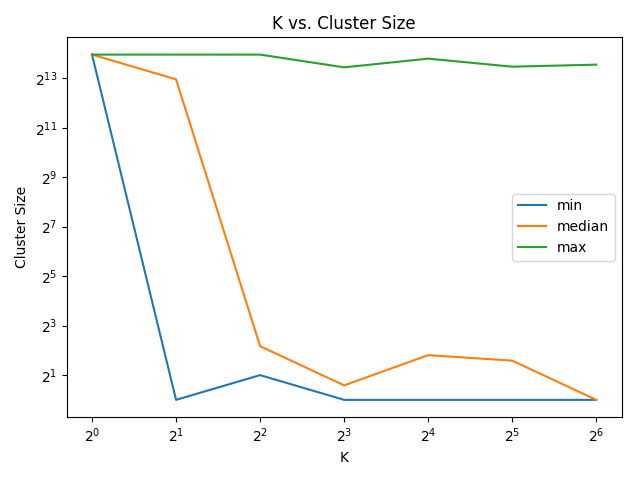
\includegraphics[scale=0.4]{k_vs_cluster_size_++}}
\end{center}
\caption{$K$ versus minimum, median, and maximum cluster size for $K \in \{1,2,4,...,64\}$ with a $log_{2}$ scale on both axes. Using K-Means++.}
\end{figure}




\section{Next Steps}

\subsection{Recursive K-Means}

One of the largest issues with applying K-Means to this dataset is that it produces clusters with huge size variations. Some clusters contain 10,000 documents, whereas others contain only one. Recursively applying K-means to large clusters could address this problem and even produce a sort of hierarchical clustering.

\subsection{Latent Dirichlet Allocation}

Some of the clusters contain documents that refer to difference meanings of the same word. For example, "season" could refer to a football season or a TV show season. I would like to explore Latent Dirichlet Allocation and whether or not it could help with this situation.

\begin{table}[t]
\caption{K-Means clusters with $K=16$ and at least 10 documents.}
\label{cluster-table}
\begin{center}
    \begin{tabular}{ | c | c | c | c |}
    \hline
    \textbf{Cluster} & \textbf{Size} & \textbf{Words} & \textbf{Documents} \\ \hline
    
0 & 10061 & \parbox[t]{2cm}{females \\ station \\ family \\ located \\ north} & \parbox[t]{8cm}{mcgillpainquestionnaire \\ historyofthefamily \\ thetussaudsgroup \\ nadiraactress \\ mansfieldsummithighschool} \\ \hline 
1 & 3013 & \parbox[t]{2cm}{church \\ college \\ students \\ published \\ institute} & \parbox[t]{8cm}{edmondscommunitycollege \\ helderbergcollege \\ oberlincongregationalchurch \\ lundbyoldchurch \\ dioceseoflimerickandkillaloe} \\ \hline 
2 & 1128 & \parbox[t]{2cm}{party \\ served \\ general \\ member \\ senate} & \parbox[t]{8cm}{partyidentification \\ labourfarmerparty \\ democraticalliancesouthafrica \\ liberaldemocratsitaly \\ christiancreditparty} \\ \hline 
3 & 909 & \parbox[t]{2cm}{season \\ club \\ playing \\ seasons \\ player} & \parbox[t]{8cm}{dancingwiththestars \\ davidmccracken \\ gilbertcurgenven \\ bjsamsamericanfootball \\ livingstonewalker} \\ \hline 
4 & 707 & \parbox[t]{2cm}{album \\ released \\ songs \\ records \\ rock} & \parbox[t]{8cm}{thegreatestdaytakethatalbum \\ conflictingemotions \\ primalscream \\ leftbacklp \\ elisamartin} \\ \hline 
5 & 30 & \parbox[t]{2cm}{nba \\ basketball \\ points \\ season \\ seasons} & \parbox[t]{8cm}{kcjones \\ hakeemolajuwon \\ albertkingbasketball \\ ballstatecardinalsmensbasketball \\ 201011southfloridabullsmensbasketballteam} \\ \hline 
6 & 23 & \parbox[t]{2cm}{riots \\ police \\ murder \\ captured \\ robbery} & \parbox[t]{8cm}{sowetouprising \\ 1992losangelesriots \\ nikolaybogolepov \\ josephlamothe \\ jenmi} \\ \hline 
7 & 13 & \parbox[t]{2cm}{congo \\ subtropical \\ republic \\ zambia \\ zimbabwe} & \parbox[t]{8cm}{republicofcabinda \\ brownrumpedbunting \\ copperbeltprovince \\ leptopelisviridis \\ yellowthroatedpetronia} \\ \hline 
 

 
\end{tabular}
\end{center}
\end{table}
\end{document}
